% Thesis: A Comparison of Base Forecasting Approaches for Spatio-Temporal Reconciliation
\input{resources/settings/settings}
\input{resources/styles/adjustments}

\usepackage{graphicx}
\usepackage{subcaption}
\usepackage{float}
\usepackage{color}
\usepackage{listings}
\usepackage{eso-pic}
\usepackage[sf]{titlesec}
\usepackage{acronym}
\usepackage[normalem]{ulem}
\usepackage{hyperref}
\usepackage{pdfpages}
\usepackage[toc,page]{appendix}
\usepackage{booktabs}
\usepackage{longtable}

\floatstyle{plaintop}
\restylefloat{table}

\hypersetup{
    colorlinks=true,
    linkcolor=black,
    filecolor=magenta,
    urlcolor=black,
    pdftitle={Master's Thesis},
    pdfpagemode=FullScreen,
    citecolor=black,
}

\interfootnotelinepenalty=10000

\newcommand\BackgroundPic{%
\put(0,0){%
\parbox[b][\paperheight]{\paperwidth}{%
\vskip 2.5cm
\centering

\includegraphics[height=1.4cm,%
keepaspectratio]{resources/images/logo_tudo.png}%
\hspace{4cm}

\includegraphics[height=1.4cm,%
keepaspectratio]{resources/images/Logo_StatistikFK.pdf}
\vfill
}}}

\makeatletter
\newcommand*{\thesisTitle}[1]{\gdef\@thesisTitle{#1}}
\newcommand*{\firstExaminer}[1]{\gdef\@firstExaminer{#1}}
\newcommand*{\secondExaminer}[1]{\gdef\@secondExaminer{#1}}
\newcommand*{\matrikelnr}[1]{\gdef\@matrikelnr{#1}}
\newcommand*{\registerDate}[1]{\gdef\@registerDate{#1}}
\newcommand*{\submitDate}[1]{\gdef\@submitDate{#1}}
\newcommand*{\courseOfStudies}[1]{\gdef\@courseOfStudies{#1}}
\newcommand*{\authorLastname}[1]{\gdef\@authorLastname{#1}}
\newcommand*{\authorFirstname}[1]{\gdef\@authorFirstname{#1}}

\renewcommand*{\maketitle}{
	\begin{titlepage}
	    \centering
		\newgeometry{left=3.5cm,right=2.5cm,top=8.2cm,bottom=1.0cm}
			\begingroup
				\fontsize{22pt}{22pt}\selectfont
				{\bfseries Master's Thesis}
			\endgroup

			\vskip 2.2cm

			\begingroup
			\fontsize{22pt}{22pt}\selectfont
			{\@thesisTitle}
			\endgroup

			\vskip 3.0cm

			\begingroup
			\fontsize{14pt}{18pt}\selectfont
				{\@authorFirstname} {\@authorLastname} \\
				Matriculation number: {\@matrikelnr} \\
				Programme: {\@courseOfStudies} \\
			\endgroup
			
			\vskip 1.0cm
			
			\begingroup
			\fontsize{14pt}{18pt}\selectfont
			    Issued on: \\
				{\@registerDate} \\
				Submitted on: \\
				{\@submitDate} \\
			\endgroup
			
			\vskip 1.2cm
			
			\begingroup
			\fontsize{12pt}{14pt}\selectfont
			    Supervisors: \\
			    {\@firstExaminer} \\
                {\@secondExaminer} \\
			\endgroup

		\restoregeometry
	\end{titlepage}
}
\makeatother


\thesisTitle{A Comparison of Base Forecasting Approaches for Spatio-Temporal Reconciliation}
\authorFirstname{[TBD]}
\authorLastname{[TBD]}
\courseOfStudies{[TBD]}
\matrikelnr{[TBD]}
\registerDate{[TBD]}
\submitDate{[TBD]}
\firstExaminer{Prof.~Dr.~Markus~Pauly}
\secondExaminer{[TBD]}

\usepackage{nomencl}
\makenomenclature
\renewcommand{\nomname}{List of Symbols}

\usepackage{fancyhdr}
\fancypagestyle{custom}{%
    \fancyhf{}
    \fancyhead[L]{\slshape\nouppercase \leftmark}
    \fancyhead[R]{\thepage}
    \renewcommand{\headrulewidth}{0.4pt}
}
\pagestyle{custom}

\begin{document}

\pagenumbering{gobble}
\AddToShipoutPicture{\BackgroundPic}
\maketitle
\newpage
\ClearShipoutPicture

\titleformat*{\section}{\Large\bfseries\sffamily}
\titleformat*{\subsection}{\bfseries\sffamily}
\titleformat*{\subsubsection}{\bfseries\sffamily}

\setlength{\parindent}{0.63cm}

% Abstract
\pagenumbering{Roman}
\section*{Abstract}
\addcontentsline{toc}{section}{Abstract}
[TBD: Context, research question, methods, key results after h=1 full run.]
\newpage

\tableofcontents
\newpage

% List of Abbreviations
\section*{List of Abbreviations}
\addcontentsline{toc}{section}{List of Abbreviations}
\begin{acronym}[CTWLSV]
 \acro{NWP}[NWP]{Numerical Weather Prediction}
 \acro{PV}[PV]{Photovoltaic}
 \acro{SARIMAX}[SARIMAX]{Seasonal Autoregressive Integrated Moving Average with eXogenous variables}
 \acro{RF}[RF]{Random Forest}
 \acro{LGBM}[LGBM]{Light Gradient Boosting Machine}
 \acro{ETS}[ETS]{Exponential Smoothing State Space model}
 \acro{CTWLSV}[CTWLSV]{Cross-Temporal Weighted Least Squares Variances reconciliation}
 \acro{CTBU}[CTBU]{Cross-Temporal Bottom-Up reconciliation}
 \acro{PERS}[PERS]{Persistence baseline forecast}
 \acro{nRMSE}[nRMSE]{normalized Root Mean Square Error}
 \acro{nMBE}[nMBE]{normalized Mean Bias Error}
 \acro{SMAPE}[SMAPE]{Symmetric Mean Absolute Percentage Error}
\end{acronym}
\newpage

% List of Symbols
\addcontentsline{toc}{section}{List of Symbols}
\nomenclature{$m$}{Seasonal period (hours per day, $m=24$)}
\nomenclature{$h$}{Forecast horizon in days}
\nomenclature{$k$}{Temporal aggregation factor}
\nomenclature{$k^*$}{Total temporal periods per day across all aggregation levels ($k^*=60$)}
\nomenclature{$\mathcal{S}$}{Spatial aggregation matrix ($324 \times 318$)}
\nomenclature{$\hat{Y}$}{Forecast vector at all temporal levels (\texttt{Y.hat})}
\nomenclature{$Y^{\mathrm{obs}}$}{Observed values}
\nomenclature{$L_0$}{Spatial hierarchy level: Total (1 series)}
\nomenclature{$L_1$}{Spatial hierarchy level: Regions (5 series)}
\nomenclature{$L_2$}{Spatial hierarchy level: Stations (318 series)}
\nomenclature{$\varepsilon$}{In-sample residuals (\texttt{Res.insamp})}
\printnomenclature
\newpage

\listoffigures
\addcontentsline{toc}{section}{List of Figures}
\newpage

\listoftables
\addcontentsline{toc}{section}{List of Tables}
\newpage

\pagenumbering{arabic}
\section{Introduction}\label{sec:introduction}

[TBD: Motivation for solar PV forecasting and spatio-temporal reconciliation.]

\subsection{Research Question}\label{sec:research-question}

This thesis addresses the following central research question:

\begin{quote}
    How do different base forecasting approaches compare when applied within the spatio-temporal reconciliation framework of \citet{difonzo2023spatiotemporal}?
\end{quote}

While \citet{difonzo2023spatiotemporal} fixed the base forecast (ETS with NWP) and compared reconciliation methods, this work reverses that design: we fix the two best-performing reconciliation methods from their study (CTWLSV and CTBU) and systematically compare eight base forecasting variants across four model families.

\subsection{Contributions}\label{sec:contributions}

[TBD after full experimental run. Planned contributions:]
\begin{itemize}
    \item A systematic comparison of statistical and machine-learning base forecasts under a common spatio-temporal hierarchy.
    \item An assessment of NWP integration strategies (integrated vs.\ L2 hourly replacement) across model families.
    \item A reproducible implementation extending the experimental setup of \citet{difonzo2023spatiotemporal}.
\end{itemize}

\subsection{Thesis Outline}\label{sec:outline}

Chapter~\ref{sec:background} reviews hierarchical forecasting and reconciliation theory.
Chapter~\ref{sec:data-design} describes the dataset, spatial and temporal hierarchy, and evaluation design.
Chapter~\ref{sec:base-methods} specifies the eight base forecasting methods.
Chapter~\ref{sec:results} presents and discusses the results.
Chapter~\ref{sec:conclusion} concludes with limitations and outlook.

\newpage
\section{Theoretical Background}\label{sec:background}

\subsection{Hierarchical Time Series}\label{sec:hierarchical-ts}

[TBD: Spatial hierarchy $L_0$, $L_1$, $L_2$; temporal aggregation levels. Cite \citet{hyndman2021fpp}, \citet{wickramasuriya2019optimal}.]

\subsection{Forecast Reconciliation}\label{sec:reconciliation-theory}

[TBD: Coherence constraints, optimal reconciliation. Brief treatment---reconciliation methods are reproduced from \citet{difonzo2023spatiotemporal}, not compared in this thesis.]

\subsection{Base Forecasting Approaches}\label{sec:base-theory}

[TBD: Overview of SARIMAX, Random Forest, LightGBM, and ETS. Cite \citet{breiman2001random}, \citet{ke2017lightgbm}, \citet{hyndman2011thief}.]

\subsection{Related Work}\label{sec:related-work}

[TBD: Yang et al.\ sequential reconciliation; Di Fonzo \& Girolimetto spatio-temporal extension \citep{difonzo2023spatiotemporal}.]

\newpage
\section{Data and Experimental Design}\label{sec:data-design}

\subsection{Dataset}\label{sec:dataset}

[TBD: \texttt{meas.csv} (318 PV stations, hourly, 365 days), \texttt{pred.csv} (NWP predictions).]

\subsection{Spatial Hierarchy}\label{sec:spatial-hierarchy}

[TBD: $L_0$ Total (1), $L_1$ Regions (5), $L_2$ Stations (318). See Figure~\ref{fig:spatial-hierarchy}.]

\begin{figure}[htbp]
    \centering
    \fbox{\parbox{0.8\textwidth}{\centering\vspace{2cm}[TBD: TikZ spatial hierarchy diagram]\vspace{2cm}}}
    \caption{Spatial hierarchy of the PV forecasting system.}
    \label{fig:spatial-hierarchy}
\end{figure}

\subsection{Temporal Aggregation}\label{sec:temporal-aggregation}

[TBD: Temporal levels $k \in \{1,2,3,4,6,8,12,24\}$, $k^*=60$. See Figure~\ref{fig:temporal-hierarchy}.]

\begin{figure}[htbp]
    \centering
    \fbox{\parbox{0.8\textwidth}{\centering\vspace{2cm}[TBD: TikZ temporal aggregation diagram]\vspace{2cm}}}
    \caption{Temporal aggregation levels from hourly ($k=1$) to daily ($k=24$).}
    \label{fig:temporal-hierarchy}
\end{figure}

\subsection{Rolling-Origin Evaluation}\label{sec:rolling-origin}

Following \citet{difonzo2023spatiotemporal}, we use a rolling-origin design with a 14-day training window (336 hours), a forecast horizon of two days (48 hourly forecasts), and 350 replications. As in the reference paper, forecast evaluation considers only the day-2 (\emph{operating day}) forecasts, consistent with operational forecast submission requirements. See Figure~\ref{fig:rolling-origin}.

\begin{figure}[htbp]
    \centering
    \fbox{\parbox{0.8\textwidth}{\centering\vspace{2cm}[TBD: TikZ rolling-origin diagram]\vspace{2cm}}}
    \caption{Rolling-origin evaluation scheme.}
    \label{fig:rolling-origin}
\end{figure}

\subsection{Reconciliation Pipeline}\label{sec:reco-pipeline}

[TBD: Two fixed reconciliation methods---CTWLSV (\texttt{FoReco::octrec}) and CTBU (\texttt{FoReco::thfrec})---reproduced from \citet{difonzo2023spatiotemporal}.]

\subsection{Evaluation Metrics}\label{sec:metrics}

[TBD: nRMSE, nMBE, Skill (vs.\ PERS), SMAPE. Formulas with nomenclature symbols.]

\newpage
\section{Base Forecasting Methods}\label{sec:base-methods}

\subsection{Pipeline Overview}\label{sec:pipeline}

[TBD: Base forecast generation $\rightarrow$ NWP post-processing (for $*$\_nwp variants) $\rightarrow$ CTWLSV/CTBU reconciliation $\rightarrow$ evaluation. See Figure~\ref{fig:pipeline}.]

\begin{figure}[htbp]
    \centering
    \fbox{\parbox{0.9\textwidth}{\centering\vspace{2cm}[TBD: TikZ pipeline diagram]\vspace{2cm}}}
    \caption{Forecasting pipeline from base methods to evaluation.}
    \label{fig:pipeline}
\end{figure}

\subsection{SARIMAX}\label{sec:method-sarimax}
[TBD: \texttt{auto.arima()} with NWP as exogenous regressor.]

\subsection{SARIMAX with NWP Replacement}\label{sec:method-sarimax-nwp}
[TBD: L2 hourly ($k=1$) replaced by NWP via post-processing.]

\subsection{Random Forest}\label{sec:method-rf}
[TBD: 500 trees, 12 features, recursive forecasting.]

\subsection{Random Forest with NWP Replacement}\label{sec:method-rf-nwp}
[TBD]

\subsection{LightGBM}\label{sec:method-lgbm}
[TBD: 300 rounds, same features as RF.]

\subsection{LightGBM with NWP Replacement}\label{sec:method-lgbm-nwp}
[TBD]

\subsection{ETS (Author Implementation)}\label{sec:method-ets-author}
[TBD: \texttt{thief:::th.forecast()} per temporal level, original author code from \citet{difonzo2023spatiotemporal}.]

\subsection{ETS (This Implementation)}\label{sec:method-ets}
[TBD: Per-level ETS with NWP hybrid at L2 hourly level.]

\newpage
\section{Results and Discussion}\label{sec:results}

\subsection{Overview}\label{sec:results-overview}

[TBD: Evaluation at $L_0$, $L_1$, $L_2$ spatial levels and hourly ($k=1$) and daily ($k=24$) temporal resolutions. Each table contains 17 rows: PERS baseline plus eight base methods reconciled via CTWLSV and CTBU.]

\subsection{Results Tables}\label{sec:results-tables}

% Auto-generated by export_thesis_tables.R from output/comparison_*.csv
\IfFileExists{tables/table_nrmse.tex}{
    \begin{table}[htbp]
\centering
\small
\caption{Mean nRMSE (\%) by base method, reconciliation approach, spatial level, and temporal resolution.}
\label{tab:nrmse}
\begin{tabular}{llrrrrrr}
\toprule
Base method & Reconciliation & L0 H & L0 D & L1 H & L1 D & L2 H & L2 D \\
\midrule
PERS & --- & 34.62 & 20.23 & 43.15 & 24.57 & 59.75 & 30.65 \\
\addlinespace
SARIMAX & CTWLSV & 30.04 & 11.28 & 35.87 & 15.33 & 52.68 & 22.44 \\
SARIMAX & CTBU & 30.66 & 11.33 & 36.39 & 15.34 & 53.08 & 22.46 \\
SARIMAX+NWP & CTWLSV & 23.82 & 10.64 & 31.33 & 14.88 & 49.29 & 22.04 \\
SARIMAX+NWP & CTBU & 23.85 & 10.59 & 31.39 & 14.82 & 49.31 & 21.99 \\
\addlinespace
RF & CTWLSV & 25.62 & 14.42 & 32.51 & 18.03 & 46.64 & 23.52 \\
RF & CTBU & 25.69 & 14.45 & 32.56 & 18.05 & 46.68 & 23.54 \\
RF+NWP & CTWLSV & 25.25 & 14.16 & 32.18 & 17.76 & 46.84 & 23.13 \\
RF+NWP & CTBU & 25.58 & 14.14 & 32.50 & 17.73 & 47.08 & 23.11 \\
\addlinespace
LightGBM & CTWLSV & 24.20 & 13.09 & 31.67 & 17.11 & 49.03 & 24.02 \\
LightGBM & CTBU & 24.34 & 13.14 & 31.75 & 17.13 & 49.08 & 24.04 \\
LightGBM+NWP & CTWLSV & 24.89 & 13.29 & 32.21 & 17.16 & 49.60 & 23.61 \\
LightGBM+NWP & CTBU & 25.71 & 13.40 & 32.86 & 17.22 & 50.04 & 23.65 \\
\addlinespace
ETS (author) & CTWLSV & 23.63 & 13.64 & 30.21 & 17.01 & 44.44 & 22.27 \\
ETS (author) & CTBU & 23.50 & 13.42 & 30.13 & 16.78 & 44.42 & 22.12 \\
ETS & CTWLSV & 23.66 & 13.68 & 30.24 & 17.04 & 44.47 & 22.29 \\
ETS & CTBU & 23.55 & 13.47 & 30.16 & 16.82 & 44.45 & 22.15 \\
\bottomrule
\end{tabular}
\end{table}


}{
    \begin{table}[htbp]
        \centering
        \caption{Mean nRMSE (\%) by method, reconciliation approach, spatial level, and temporal resolution. [Run \texttt{export\_thesis\_tables.R} after evaluation.]}
        \label{tab:nrmse}
        \fbox{\parbox{0.9\textwidth}{\centering\vspace{1cm}Table not yet generated.\vspace{1cm}}}
    \end{table}
}

\IfFileExists{tables/table_nmbe.tex}{\begin{table}[htbp]
\centering
\small
\caption{Mean nMBE (\%) by base method, reconciliation approach, spatial level, and temporal resolution.}
\label{tab:nmbe}
\begin{tabular}{llrrrrrr}
\toprule
Base method & Reconciliation & L0 H & L0 D & L1 H & L1 D & L2 H & L2 D \\
\midrule
PERS & --- & -0.08 & -0.08 & -0.06 & -0.06 & -0.08 & -0.08 \\
\addlinespace
SARIMAX & CTWLSV & -3.33 & -3.33 & -3.10 & -3.10 & -3.41 & -3.41 \\
SARIMAX & CTBU & -3.49 & -3.49 & -3.24 & -3.24 & -3.57 & -3.57 \\
SARIMAX+NWP & CTWLSV & -1.44 & -1.44 & -1.40 & -1.40 & -1.47 & -1.47 \\
SARIMAX+NWP & CTBU & -1.25 & -1.25 & -1.18 & -1.18 & -1.28 & -1.28 \\
\addlinespace
RF & CTWLSV & -2.66 & -2.66 & -2.56 & -2.56 & -2.69 & -2.69 \\
RF & CTBU & -2.72 & -2.72 & -2.63 & -2.63 & -2.75 & -2.75 \\
RF+NWP & CTWLSV & -1.70 & -1.70 & -1.65 & -1.65 & -1.72 & -1.72 \\
RF+NWP & CTBU & -1.63 & -1.63 & -1.58 & -1.58 & -1.64 & -1.64 \\
\addlinespace
LightGBM & CTWLSV & -1.29 & -1.29 & -1.24 & -1.24 & -1.31 & -1.31 \\
LightGBM & CTBU & -1.35 & -1.35 & -1.29 & -1.29 & -1.37 & -1.37 \\
LightGBM+NWP & CTWLSV & 0.24 & 0.24 & 0.23 & 0.23 & 0.23 & 0.23 \\
LightGBM+NWP & CTBU & 0.31 & 0.31 & 0.31 & 0.31 & 0.31 & 0.31 \\
\addlinespace
ETS (author) & CTWLSV & 1.31 & 1.31 & 1.20 & 1.20 & 1.34 & 1.34 \\
ETS (author) & CTBU & 1.43 & 1.43 & 1.32 & 1.32 & 1.45 & 1.45 \\
ETS & CTWLSV & 1.42 & 1.42 & 1.30 & 1.30 & 1.45 & 1.45 \\
ETS & CTBU & 1.57 & 1.57 & 1.45 & 1.45 & 1.60 & 1.60 \\
\bottomrule
\end{tabular}
\end{table}

}{}
\IfFileExists{tables/table_skill.tex}{\begin{table}[htbp]
\centering
\small
\caption{Mean Skill score (\%) relative to PERS by base method, reconciliation approach, spatial level, and temporal resolution.}
\label{tab:skill}
\begin{tabular}{llrrrrrr}
\toprule
Base method & Reconciliation & L0 H & L0 D & L1 H & L1 D & L2 H & L2 D \\
\midrule
PERS & --- & 0.00 & 0.00 & 0.00 & 0.00 & 0.00 & 0.00 \\
\addlinespace
SARIMAX & CTWLSV & 13.23 & 44.24 & 17.53 & 37.79 & 12.29 & 27.08 \\
SARIMAX & CTBU & 11.44 & 44.01 & 16.24 & 37.71 & 11.61 & 27.01 \\
SARIMAX+NWP & CTWLSV & 31.20 & 47.41 & 27.51 & 39.50 & 17.86 & 28.42 \\
SARIMAX+NWP & CTBU & 31.09 & 47.68 & 27.26 & 39.71 & 17.81 & 28.58 \\
\addlinespace
RF & CTWLSV & 25.99 & 28.72 & 24.66 & 26.62 & 22.05 & 23.31 \\
RF & CTBU & 25.80 & 28.59 & 24.54 & 26.55 & 21.98 & 23.25 \\
RF+NWP & CTWLSV & 27.05 & 30.03 & 25.45 & 27.74 & 21.75 & 24.60 \\
RF+NWP & CTBU & 26.11 & 30.13 & 24.71 & 27.89 & 21.35 & 24.69 \\
\addlinespace
LightGBM & CTWLSV & 30.10 & 35.29 & 26.49 & 30.32 & 17.95 & 21.57 \\
LightGBM & CTBU & 29.69 & 35.05 & 26.30 & 30.23 & 17.86 & 21.52 \\
LightGBM+NWP & CTWLSV & 28.09 & 34.32 & 25.17 & 30.10 & 17.03 & 22.98 \\
LightGBM+NWP & CTBU & 25.73 & 33.74 & 23.61 & 29.89 & 16.29 & 22.85 \\
\addlinespace
ETS (author) & CTWLSV & 31.75 & 32.58 & 30.05 & 30.85 & 25.81 & 27.51 \\
ETS (author) & CTBU & 32.12 & 33.67 & 30.24 & 31.82 & 25.85 & 28.02 \\
ETS & CTWLSV & 31.64 & 32.40 & 30.00 & 30.73 & 25.77 & 27.44 \\
ETS & CTBU & 31.98 & 33.41 & 30.17 & 31.63 & 25.80 & 27.91 \\
\bottomrule
\end{tabular}
\end{table}

}{}
\IfFileExists{tables/table_smape.tex}{\begin{table}[htbp]
\centering
\small
\caption{Mean SMAPE (\%) by base method, reconciliation approach, spatial level, and temporal resolution.}
\label{tab:smape}
\begin{tabular}{llrrrrrr}
\toprule
Base method & Reconciliation & L0 H & L0 D & L1 H & L1 D & L2 H & L2 D \\
\midrule
PERS & --- & 10.86 & 7.75 & 12.94 & 9.78 & 20.20 & 13.05 \\
\addlinespace
SARIMAX & CTWLSV & 57.50 & 4.85 & 58.30 & 6.69 & 56.90 & 10.07 \\
SARIMAX & CTBU & 57.69 & 4.89 & 58.56 & 6.71 & 58.56 & 10.09 \\
SARIMAX+NWP & CTWLSV & 56.25 & 4.46 & 57.25 & 6.36 & 54.19 & 9.74 \\
SARIMAX+NWP & CTBU & 56.33 & 4.42 & 57.40 & 6.31 & 54.09 & 9.70 \\
\addlinespace
RF & CTWLSV & 54.20 & 5.80 & 55.54 & 7.59 & 51.77 & 10.34 \\
RF & CTBU & 54.24 & 5.82 & 55.57 & 7.60 & 51.96 & 10.35 \\
RF+NWP & CTWLSV & 54.67 & 5.62 & 55.99 & 7.41 & 51.05 & 10.10 \\
RF+NWP & CTBU & 55.15 & 5.61 & 56.60 & 7.39 & 51.48 & 10.08 \\
\addlinespace
LightGBM & CTWLSV & 55.59 & 5.29 & 56.82 & 7.21 & 55.36 & 10.52 \\
LightGBM & CTBU & 55.64 & 5.31 & 56.86 & 7.22 & 55.58 & 10.53 \\
LightGBM+NWP & CTWLSV & 55.85 & 5.28 & 57.14 & 7.12 & 53.96 & 10.23 \\
LightGBM+NWP & CTBU & 56.26 & 5.31 & 57.60 & 7.13 & 54.69 & 10.24 \\
\addlinespace
ETS (author) & CTWLSV & 55.18 & 5.31 & 56.26 & 6.95 & 47.27 & 9.55 \\
ETS (author) & CTBU & 55.43 & 5.24 & 56.45 & 6.86 & 47.45 & 9.48 \\
ETS & CTWLSV & 55.34 & 5.32 & 56.59 & 6.95 & 52.19 & 9.55 \\
ETS & CTBU & 55.64 & 5.25 & 56.95 & 6.87 & 52.90 & 9.48 \\
\bottomrule
\end{tabular}
\end{table}

}{}

\subsection{Discussion}\label{sec:discussion}

[TBD after h=1 full run:]
\begin{itemize}
    \item Overall ranking across spatial and temporal levels
    \item Effect of NWP variants within each model family
    \item Sensitivity to reconciliation method (CTWLSV vs.\ CTBU)
    \item Comparison to the ETS+NWP baseline of \citet{difonzo2023spatiotemporal}
\end{itemize}

\subsection{Limitations}\label{sec:limitations}

[TBD: Single dataset, deterministic forecasts, replication constraints.]

\newpage
\section{Conclusion}\label{sec:conclusion}

\subsection{Summary}\label{sec:summary}

[TBD: Answer to the research question. Best-performing base methods per hierarchy level.]

\subsection{Outlook}\label{sec:outlook}

[TBD: Additional base methods, probabilistic forecasts, other datasets, alternative reconciliation approaches.]

\newpage

\addcontentsline{toc}{section}{Bibliography}
\bibliography{literatur}

\begin{appendices}

\section{Reconciliation Implementation}\label{app:reconciliation}

[TBD: CTWLSV and CTBU details, FoReco format transformation. See repository \texttt{docs/RECONCILIATION\_METHODS.md}.]

\section{Replication Bug Fixes}\label{app:bug-fixes}

[TBD: File loading order and FoReco format mismatch. See \texttt{docs/BUG\_FIXES.md}.]

\section{Supplementary Results}\label{app:supplementary}

[TBD: Optional intermediate temporal levels, example forecast plot.]

\end{appendices}

\newpage

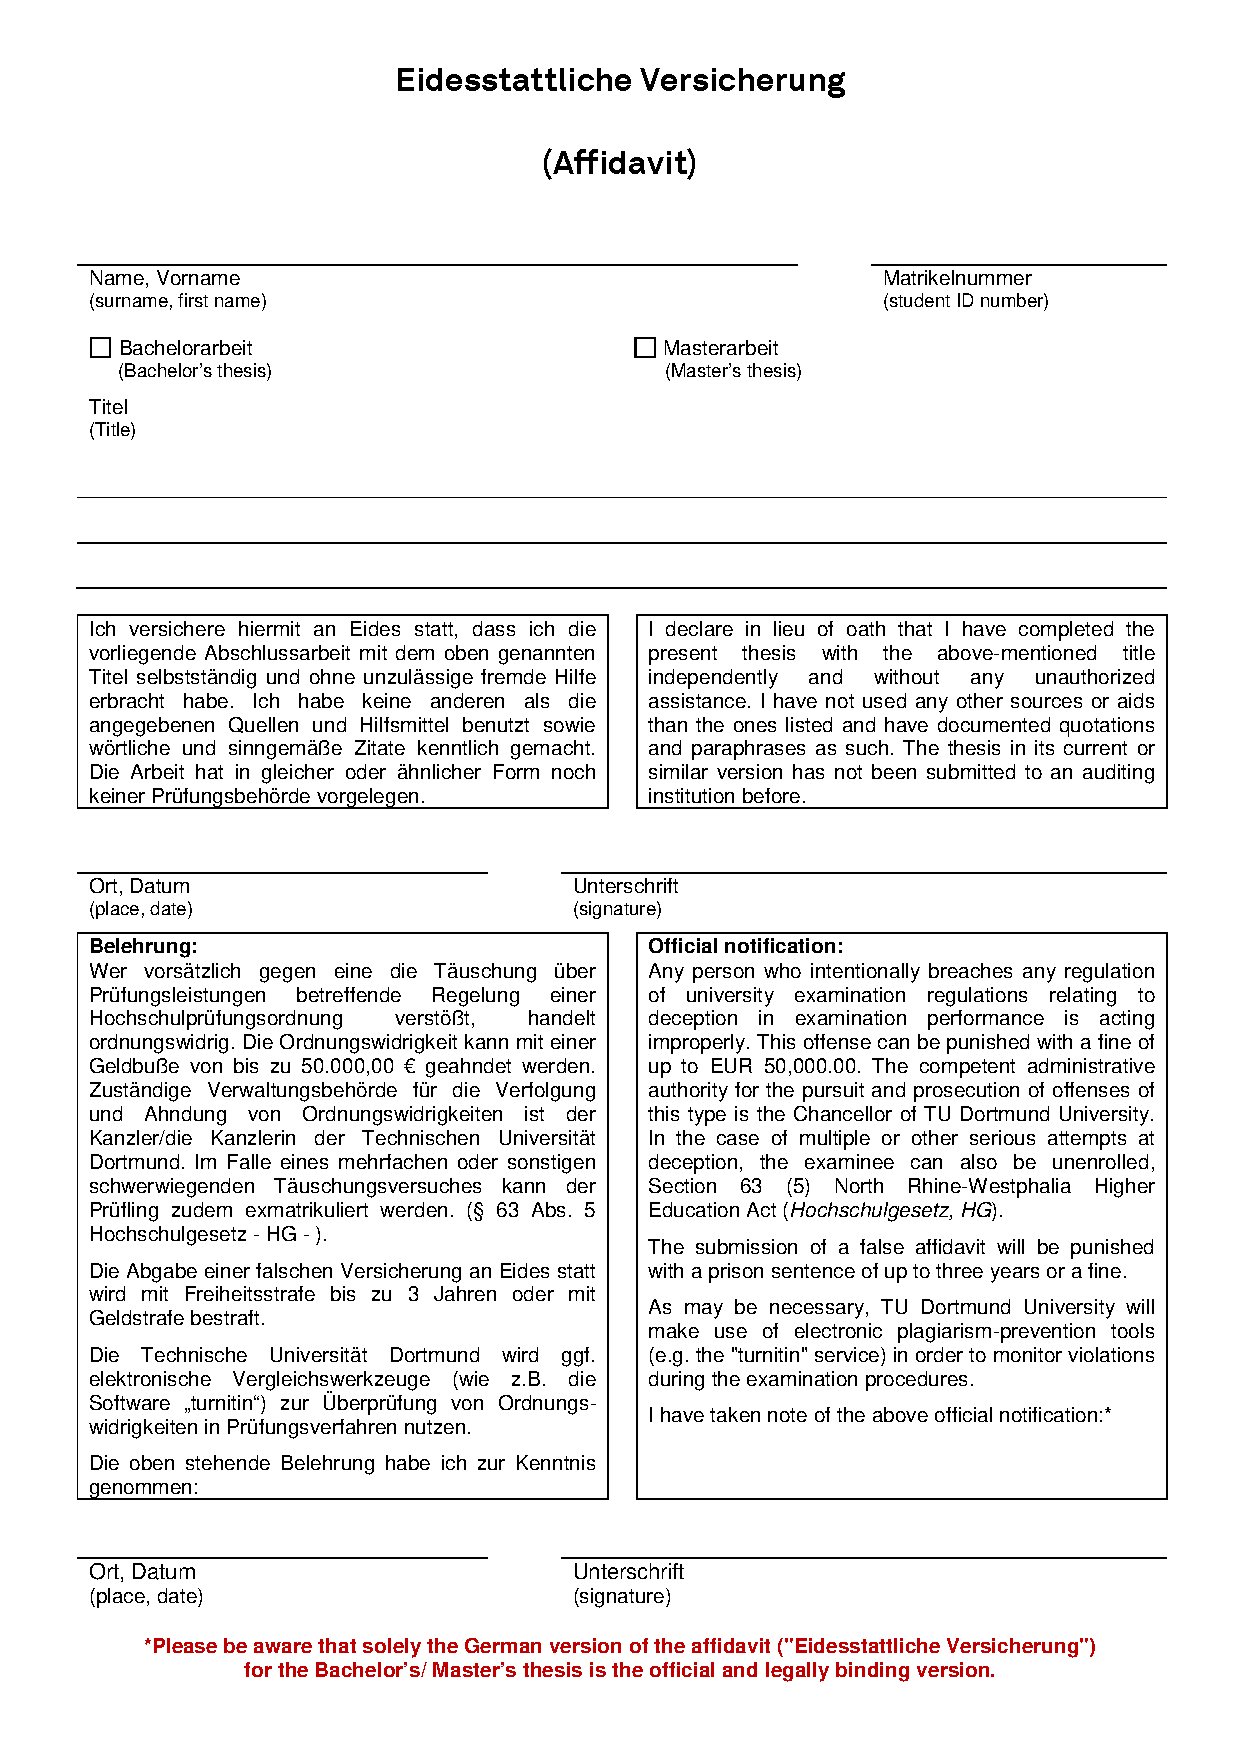
\includepdf[pages={1}]{resources/Eidesstattliche_Versicherung.pdf}

\end{document}
